%% pfgguide.dtx Copyright (c) 1995 Michael C. Grant and Craig Barratt
%%              All rights are reserved.
%%
%%            This system is distributed in the hope that it will be
%%            useful, but WITHOUT ANY WARRANTY; without even the
%%            implied warranty of MERCHANTABILITY or FITNESS FOR A
%%            PARTICULAR PURPOSE. Don't come complaining to us if you
%%            modify this file and it doesn't work! If this file is
%%            modified by anyone but the authors, those changes and
%%            their authors must be explicitly stated HERE.
%%
%%              Modificato da Flavio Casadei Della Chiesa
%%              Modifiche: traduzione in Italiano
\documentclass[a4paper,11pt]{ltxguide}
\usepackage{shortvrb,psfrag,graphicx}
%% ho agiunto il babel (italian) ed ndt
\usepackage[italian]{babel}
\newcommand{\ndt}[1]{\footnote{#1 [N.d.T.]}}
\usepackage{hyperref}
% I prefer more to a page.
\marginparsep 0pt \oddsidemargin 0pt \evensidemargin 0pt
\textwidth \paperwidth \advance \textwidth by-2in
\topmargin 0pt \headheight 0pt \headsep 0pt
\textheight \paperheight \advance \textheight by-2in

\let\pkg\textsf
\let\fname\texttt
\let\pscom\texttt
\newcommand{\pfg}{\pkg{PSfrag}}
% cambiati newcomamnd  in renewcommand
%\renewcommand{\ie}{\emph{cio\`e\@}}
%\renewcommand{\eg}{\emph{e.g.\@}}
% tutto come prima
\newcommand{\etc}{\emph{etc.\@}}
\newcommand{\netaddress}[1]{\texttt{#1}}
\MakeShortVerb{\|}
\def\cs#1{%
  {\ttfamily\expandafter\string\csname #1\endcsname}}
\providecommand\marg[1]{%
  {\ttfamily\char`\{}{\em#1\/}{\ttfamily\char`\}}}
\providecommand\oarg[1]{%
  {\ttfamily[}{\em #1\/}{\ttfamily]}}
\providecommand\parg[1]{%
  {\ttfamily(}{\em #1\/}{\ttfamily)}}

\title{Il sistema \pfg, versione 3}
\author{Michael C. Grant \and David Carlisle\\
        \netaddress{psfrag@rascals.stanford.edu}\ndt{Questo indirizzo 
non \`e pi\`u attivo}}
\date{11 Aprile 1998}

\begin{document}

\maketitle
\begin{center}
Tradotto da FLavio Casadei Della Chiesa e Lorenzo Masetti
\end{center}
\tableofcontents

%\section{What is \pfg?}
\section{Cosa \`e \pfg?}

Molti pacchetti di grafica e disegno producono output nel formato
Encapsulated PostScript (EPS), ma pochi possono facilmente produrre
equazioni e testi scientifici nei quali \TeX\  \`e cos\`{\i}
abile. D'altro canto, la maggior parte dei pacchetti per grafica
basati su \LaTeX{}  non \`e cos\`{\i} espressiva e di facile
utilizzo come questi strumenti \emph{stand-alone}.

\pfg\ fornisce il meglio dei due mondi, permettendo all'utente di
arricchire file Encapsulated PostScript (EPS) con costrutti
\LaTeX{} arbitrari.
Per compiere questo, l'utente piazza un semplice \emph{tag} 
di testo
nel file grafico, come una sorta di marcatore di posizione. 
Quindi, utilizzando semplici comandi \LaTeX{}, l'utente ordina a
 \pfg\ di rimuovere quel \emph{tag} dalla figura, e di sostituirlo con
un'equazione \LaTeX{} opportunamente ridimensionata, allineata e ruotata.
\pfg\ permette all'utente di inserire costrutti \LaTeX{} direttamente 
nello stesso file EPS. 

Il Dott.~Craig Barrat scrisse la versione originale di \pfg\ quando
era studente presso la Stanford University. 
Da allora l'interfaccia
\`e cambiata solo leggermente, ma l'implementazione \`e stata completamente
riscritta. La versione attuale di \pfg{} viene mantenuta da Michael Grant
e David Carlisle. Si ringraziano i membri della mailing
list di \pfg{}, e chiunque abbia 
inviato segnalazioni di bug o suggerimenti.

%%% Nota del traduttore
\subsubsection*{Nota alla traduzione italiana}
Una copia di questo documento e altre traduzioni in italiano di
manuali \LaTeX\ sono reperibili presso:
\begin{itemize}
\item\url{http://guild.prato.linux.it}
\item\url{ftp://lorien.prato.linux.it/pub/guild}
\end{itemize}
e su ogni sito CTAN nella directory \url{/info/italian}.  Per un
elenco aggiornato dei siti mirror CTAN consultate
\url{http://www.ctan.org/} alla voce ``CTAN mirror''.
%%%%%%%%%%%%%%%%%%%%%%%%%%%%%%%%%%%%%%%%%%%%%%%%%%%%%%%%%%%%%%%%%%%%%%%%






\section{Cosa serve a \pfg}

Per utilizzare \pfg\ sono necessari i seguenti tool:
\begin{itemize}
\item Una versione recente di \LaTeXe\ e del pacchetto \pkg{graphics}.
  \pfg\ richiede la versione del 01/12/1997 o superiore di entrambi i
  pacchetti, comunque \`e sempre meglio avere le versioni pi\`u 
  recenti.
\item Se si pensa di utilizzare il pacchetto \pkg{seminar} con  \pfg\ 
  \`e necessario assicurarsi di avere la versione del 13/10/1997 
  o superiore (controllare il paragrafo~\ref{sec:sem-bug}).
\end{itemize}

Le ultime versioni di \LaTeXe, del pacchetto \pkg{graphics}, di \pfg, 
e di \pkg{dvips} possono essere trovate sul CTAN, il Comprehensive \TeX\ 
Archive Network. I siti CTAN ed i loro mirror includono:
\begin{center}
  \begin{tabular}{lll}
    Nome & Indirizzo IP  & Locazione \\ \hline
    |ftp.dante.de| & 129.206.100.192 & Germania \\
    |ftp.tex.ac.uk| & 128.232.1.87 & Regno Unito \\
    |ftp.cdrom.com| & 165.113.58.253 & USA \\
  \end{tabular}
\end{center}

\subsection{Scelta di un \emph{driver} PostScript}
\label{sec:compat}

\pfg\ si basa su qualche ``trucco'' PostScript per raggiungere i suoi scopi.
A causa di tempo e risorse limitate, l'autore non pu\`o confermare che
\pfg\ funzioni correttamente con ogni \emph{driver} PostScript disponibile. Abbiamo
tentato di assicurare che col tempo \pfg\ funzioner\`a con ogni \emph{driver} 
pienamente compatibile con il pacchetto \pkg{graphics} 
(ovvero uno con il quale viene fornito un file \fname{.def}.) 

\`E stato confermato che \pfg\  funziona con i seguenti \emph{driver}:
\begin{center}
\begin{tabular}{lll}
\emph{Driver} & Testato da & Compatibilit\`a \\ \hline
Thomas Rokicki's \pkg{dvips} & gli autori &
pienamente compatibile \\
Y\&Y's \pkg{DVIPSONE} & gli autori &
pienamente compatibile
\end{tabular}
\end{center}

Aiutateci ad aggiungere campi a questa lista! Se  \pfg\ funziona
con il vostro \emph{driver} fatecelo sapere, in questo modo possiamo aggiungerlo alla
lista. Se possibile, verificate l'output %di \pfg, ma non lo inserirei
sia su stampanti Level~1 che Level~2, in modo da poter fare eventuali
distinzioni se necessario. Se \pfg\ non funziona, per favore inviate una
segnalazione del bug; consultate il paragrafo~\ref{sec:mail} per sapere
come contattarci. Sfortunatamente, non possiamo promettere un rimedio
per tutti, ma ci piacerebbe assicurare che i \emph{driver} pi\`u popolari
rimangano compatibili.

\section{Installare \pfg}

Installare i vari file del \pfg\ \`e semplicissimo:
\begin{enumerate}
\item Eseguire \LaTeX{} su \fname{psfrag.ins} per estrarre
  \fname{psfrag.sty} e \fname{psfrag.pro}
\item Installare \fname{psfrag.sty} nella locazione usuale
  per le macro di \LaTeX{}. In distribuzioni basate su \pkg{kpathsea}
  tipo \pkg{te\TeX}, questa locazione \`e determinata dalla variabile
  \texttt{TEXINPUTS}.
\item Installare \fname{psfrag.pro} dove il \emph{driver} PostScript va a 
  cercare i file di intestazione. Per sistemi basati su \pkg{kpathsea} tipo 
  \pkg{te\TeX}, questo \`e indicato dalla variabile \texttt{DVIPSHEADERS}.
  Per  \pkg{dvips}, in particolare, la scelta pi\`u sensata \`e la 
  stessa directory dei file \fname{tex.pro} e \fname{special.pro}.
\item Se si possiede una vecchia versione di \pfg, bisogna cancellare,
        se esistono, i seguenti file: \fname{ps2frag.ps}, \fname{ps2frag},
   \fname{ps2psfrag} (i vari script di eleborazione), e \fname{epsf.sty}
  (quello fornito da \pfg{}, \emph{non} quello di \pkg{dvips}!). 
  Gli amministratori di sistema dovrebbero sostituire \fname{ps2frag}
  con uno script che avverta gli  utenti dell'aggiornamento.
\end{enumerate}

\section{Utilizzo}
Qua sotto c'\`e una veloce descrizione dell'utilizzo di \pfg{}:
\begin{itemize}
  
\item Usare il comando \cs{includegraphics} definito dai pacchetti
  \pkg{graphics} e \pkg{graphicx} per aggiungere figure EPS. Se si
  utilizza il comando \cs{epsfbox} di \fname{epsf.sty}, allora
  \fname{epsf.sty} deve essere caricato dopo \fname{psfrag.sty}. Altri
  pacchetti basati su \fname{graphics.sty}, tipo \pkg{graphicx} oppure
  \pkg{epsfig}, non soffrono di questa restrizione.

\item Caricare \fname{psfrag.sty} con un comando \cs{usepackage}.
  
\item Assicurarsi che le figure EPS contengano un semplice \emph{tag}
  in ciascuna delle posizioni in cui si vuole mettere un comando
  \LaTeX{}. Bisogna utilizzare una sola parola composta da
  lettere non accentate e numeri. Si \`e cercato di permettere
  l'utilizzo di un \emph{tag} di testo pi\`u arbitrario, ma il
  meccanismo non \`e infallibile; si veda il paragrafo~\ref{sec:tags}.
%
%\item Make sure that your EPS figures contain a simple ``tag'' word in
%          each position that you would like a \LaTeX{} replacements. Use
%          a \emph{single} word, composed of unaccented letters and numbers. 
%          Some effort has been made to allow for more arbitrary tag text, 
%          but the mechanism is not infallible; see section \ref{sec:tags}.
  
\item Per ogni \emph{tag} nel file EPS, aggiungere un comando al
  documento \LaTeX{} per specificare in che modo questo \emph{tag}
  debba essere sostituito, nel modo seguente:
\begin{quote}
    \cs{psfrag}\marg{tag}\oarg{posn}\oarg{psposn}%
    \oarg{scala}\oarg{rot}\marg{testo \LaTeX{} }
\end{quote}

Il \emph{tag} verr\`a sostituito con del testo \LaTeX{}.
Per esempio: in un programma di disegno tipo \pkg{xfig}, piazzare
il testo
\begin{quote}
        |xy|
\end{quote}
in un punto particolare. Per sostituirlo con $x+y$, si pu\`o usare la macro 
\begin{quote}
            \cs{psfrag{xy}{$x+y$}}
\end{quote}

\end{itemize}

Tutte le chiamate a comandi \cs{psfrag} che precedono \cs{includegraphics}
(o comandi equivalenti) nello stesso ambiente o in ambienti circostanti
verranno utilizzate solo per un dato file EPS; in questo modo
possono essere definiti sia comandi \cs{psfrag} ``globali'' che locali ad una 
certa figura.

Qualsiasi testo che non viene menzionato in un comando \cs{psfrag} non
verr\`a sostituito, quindi PostScript e \LaTeX{} possono essere
liberamente mescolati.  Visualizzando l'output con un visualizzatore
DVI tipo \pkg{xdvi} o \pkg{dviwin}, una lista verticale delle
sostituzioni effettuate verr\`a piazzata a sinistra di ciascuna
figura.  Essa permette di controllare la formattazione delle
sostituzioni, e comunque scompare nel documento PostScript finale.
Sfortunatamente i \emph{driver} DVI non sono capaci di piazzare le
sostituzioni effettuate da \pfg{} sopra le figure e quindi per vedere
il risultato \`e necessario stampare oppure utilizzare un
visualizzatore PostScript tipo GhostView.

Questa versione del \pfg\ dovrebbe funzionare in modo adeguato
nella modalit\`a di compatibilit\`a \LaTeX2.09. 

\section{Comandi e ambienti}\label{sec:pos}

\begin{decl}
\cs{psfrag}\marg{tag}\oarg{posn}\oarg{psposn}%
        \oarg{scala}\oarg{rot}\marg{sostituzione}\\
\cs{psfrag*}\marg{tag}\oarg{posn}\oarg{psposn}%
        \oarg{scala}\oarg{rot}\marg{sostituzione}
\end{decl}

%orrenda
La macro \cs{psfrag} definisce una ``\marg{sostituzione} \LaTeX{}''  che deve
essere piazzata al posto dei \marg{tag} PostScript. Il comando
deve essere inserito prima della chiamata ad \cs{includegraphics}, o comandi
equivalenti, ed ha effetto su tutte le occorrenze del \marg{tag} nella
figura. 
% ORRENDO Controllare please
%The \cs{psfrag} macro defines a \LaTeX-typeset \marg{replacement} to be placed
%at the same position as a PostScript \marg{tag}. The command should be placed
%before the call to \cs{includegraphics}, or equivalent. It matches \emph{all}
%occurrences of \marg{tag} in the figure.

Un comando \cs{psfrag} rimarr\`a attivo fino alla chiusura dell'ambiente
in cui \`e stato invocato.
Si possono perci\`o definire \cs{psfrag} globali, che vengono
applicati ad ogni figura, o, ad esempio, un \cs{psfrag} all'interno di
un ambiente |figure| in modo che venga applicato ad un solo
file EPS.

Gli argomenti opzionali di posizionamento \oarg{posn} e \oarg{pspons}
specificano come vengono allineati il \emph{bounding box} del testo
\LaTeX{} ed il \emph{bounding box} del testo PostScript,
rispettivamente.  Alcuni strumenti per disegnare potrebbero chiamare
questi oggetti \emph{control point} o \emph{alignment point}.
% help control points alignment point

\begin{description}
\item{\oarg{posn}} il punto di riferimento di \LaTeX{}.  La sintassi
  di questo argomento \`e identica a quella del comando \cs{makebox}.
  Possono essere scelte fino a due lettere, una dalla lista
  \{|t|,|b|,|B|,|c|\} (in cima, in fondo, sulla \emph{baseline}, al
  centro) e l'altra dalla lista \{|l|,|r|,|c|\} (a sinistra, a destra,
  al centro). Se una delle due manca, viene utilizzato |c| (centro).
  Assieme, esse specificano uno dei 12 punti di ancoraggio; se
  l'argomento viene interamente omesso, allora viene assunto
  |[Bl]|---ma nota che fornendo |[]| si intende posizionamento
  centrato.
  
  Quando utilizzato nella modalit\`a di compatibilit\`a \LaTeX{}2.09,
  l'allineamento predefinito \`e |[bl]|, questo per supportare i
  vecchi documenti.  Di solito non dovrebbe essere una
  differenza significativa.
  
\item{\oarg{psposn}} Il punto di riferimento del testo PostScript. I
  possibili argomenti sono identici a quelli del \oarg{posn}, lo
  stesso dicasi per il valore predefinito, |[Bl]| (|[bl]| nella
  modalit\`a di compatibilit\`a \LaTeX{}2.09).
\end{description}

La sostituzione \LaTeX{} pu\`o essere opzionalmente ridimensionata 
%scalata
e ruotata rispetto al suo punto di riferimento:
\begin{description}
\item{\oarg{scala}} Fattore di scala.  \`E meglio utilizzare il
  cambiamento della dimensione dei font nel testo \LaTeX{} piuttosto
  che il fattore di scala, ma si pu\`o utilizzare il fattore di scala
  per aggiustare la loro dimensione. Il valore predefinito \`e |[1]|.
\item{\oarg{rotn}} Rotazione aggiuntiva attorno al punto di
  riferimento, in gradi. La rotazione ``nominale'' del testo \LaTeX{}
  combacia con quella del testo PostScript che deve sostituire; la
  rotazione totale \`e questo valore ``nominale'' pi\`u \oarg{rotn}.
  Il valore predefinito \`e |[0]|.
\end{description}

\begin{figure}[tbh]
\psfragdebugon
\begin{center}
     \psfrag{gA}[br][br]{|[br][br]|}
     \psfrag*{gA}[Br][b ][2]{|[Br][b][2]|}
     \psfrag*{gA}[ r][bl]{|[r][bl]|}
     \psfrag*{gA}[tr][Bl]{|[tr][Bl]|}
     \psfrag*{gA}[b ][B ]{|[b][B]|}
     \psfrag*{gA}[B ][Br]{|[B][Br]|}
     \psfrag*{gA}[  ][ r]{|[][r]|}
     \psfrag*{gA}[t ][  ][0.75][45]{|[t][][0.75][45]|}
     \psfrag*{gA}[bl][ l][1.5][30]{|[bl][l][1.5][30]|}
     \psfrag*{gA}[Bl][tl]{|[Bl][tl]|}
     \psfrag*{gA}[bl][Bl]{~~~~~(\emph{baseline})}
     \psfrag*{gA}[bl][l]{~~~~~(linea centrale)}
     \psfrag*{gA}[bl][t][1][-90]{~~~~~(linea centrale)}
     \psfrag*{gA}[ l][t ]{|[l][t]|}
     \psfrag*{gA}[tl][tr][1][180]{|[tl][tr][1][180]|}
     \resizebox{4in}{!}{\includegraphics[angle=30]{testfig.eps}}
\end{center}
\caption{Una dimostrazione delle varie opzioni per il comando \cs{psfrag}.}
\label{fig:argexam}
\end{figure}
La figura~\ref{fig:argexam} illustra varie combinazioni di argomenti.
Se si visualizza questo documento con un visualizzatore DVI tipo
\pkg{xdvi}, allora le sostituzioni \pfg{} dovrebbero essere allineate
alla sinistra della figura e, se il visualizzatore \`e capace di
mostrare file EPS, si dovrebbe vedere una grande |gA| ruotata.  Se si
stampa il documento, o se lo si visualizza con un visualizzatore
PostScript come GhostView, allora le sostituzioni dovrebbero essere
sovrapposte su una rappresentazione grafica del \emph{bounding box},
linee centrali e \emph{baseline} del \emph{tag} |gA|. (La
rappresentazione grafica dei \emph{bounding box} \`e fornita solo in
modalit\`a debug.)

Se \`e gi\`a stata definita una sostituzione per \marg{tag}, allora il
comando \cs{psfrag} senza asterisco lo sostituir\`a senza avvertire.
La versione asteriscata, comunque, aggiunger\`a una nuova
sostituzione alla lista. Utilizzando la versione asteriscata, un solo
pezzo di un testo PostScript pu\`o innescare molte sostituzioni. Non
mi viene in mente il motivo per cui molti utenti utilizzano la
versione asteriscata del comando, comunque nella
figura~\ref{fig:argexam} \`e stata utilizata a titolo esemplificativo.


\begin{decl}
\cs{begin}|{psfrags}|
\cs{end}|{psfrags}|
\end{decl}

Si pu\`o utilizzare l'ambiente |psfrag| per delimitare la visibilit\`a
%(lo scope, in informatica di traduce cosi')
delle chiamate a \cs{psfrag}.  Come detto sopra, i comandi \cs{psfrag}
persistono fino all'uscita dal pi\`u vicino ambiente circostante.
\emph{Qualsiasi} ambiente: |center|, |figure|, etc., quindi non
dovrebbe essere necessario utilizzare questo ambiente, che non ha
altri effetti sul documento.


\subsection{Inglobare operazioni \pfg\ nei file EPS}
\label{sec:texcomm}

\begin{decl}
\cs{tex}\oarg{posn}\oarg{psposn}\oarg{scala}%
        \oarg{rot}\marg{\LaTeX\ text}\\
\cs{psfragscanon}~~~\cs{psfragscanoff}
\end{decl}

\pfg\ 3.0 supporta i comandi ``incorporati'' \cs{tex} che si trovano
anche nella precedente versione di \pfg. Usati propriamente sono uno
strumento potentissimo, ma sono stati deprecati a causa della
necessit\`a di un passo di \emph{pre-processing}.
Diversamente dalle precedenti versioni di \pfg, il supporto per il
comando \cs{tex} deve essere esplicitamente dichiarato, come
descritto qua sotto.

Come si pu\`o vedere, la sintassi del comando \cs{tex} \`e molto
simile a quella del comando \cs{psfrag}, solo che, invece di inserire
il comando \cs{tex} nel file \LaTeX{}, il comando \cs{tex} \`e
incorporato nel file EPS stesso.  In altre parole, il comando
diventa il \emph{tag} di sostituzione.

Per esempio, si pu\`o piazzare il testo
\begin{quote}
    |\tex[bl][bl]{$\alpha$}|
\end{quote}
in un punto particolare del file EPS per fare in modo che il \LaTeX{}
lo sostituisca con $\alpha$. Molti utenti \pfg\ trovano questa
funzionalit\`a utile per etichettare gli assi cartesiani, titoli e
legende nei grafici MATLAB.

Il vantaggio di questo approccio \`e che i cambiamenti possono essere
fatti direttamenti nel file EPS senza dover modificare alcun comando 
\cs{psfrag} nel file LaTeX. (\`E comunque necessario ricompilare
il file \LaTeX{} in questi casi.)

Ci sono comunque svantaggi e avvertimenti in questo tecnica, che includono:
\begin{itemize}
\item Per cambiare le etichette create dai comandi \cs{tex} si deve
  modificare la figura; invece se si utilizza \cs{psfrag}, bisogna
  solamente modificare il documento, il che pu\`o essere meno
  faticoso. (Si deve comunque eseguire \LaTeX{} in entrambi i casi.)
\item Dato che i comandi \cs{tex} sono lunghe stringhe di caratteri, essi 
        possono alterare il \emph{bounding box} in modo
        indesiderato. Questo problema pu\`o essere mitigato riducendo la 
        dimensione del font della stringa \cs{tex}, dato che non ha effetto
        sulla dimensione della sostituzione del \pfg.
\item Il comando \cs{tex} non \`e supportato da documenti PostScript 
        compressi.
\item Il motore \TeX{} deve scandire il file EPS per trovare queste
        stringhe, e questo potrebbe aumentare il tempo di eleborazione
        del documento. (Ad essere onesti, 
        non abbiamo ancora incontrato un caso in
        cui questo ritardo diventa rilevante.)    
\item Importante: ogni volta che un file viene scandito da \pfg, si genera
        un file \fname{nomefile.pfg}, dove \fname{nomefile} 
        \`e il nome del file principale del documento \LaTeX{}. 
        Ogni file con lo stesso nome verr\`a sovrascritto 
        senza avvertimento.
\end{itemize}

Questa funzionalit\`a non viene da tempo abilitata in automatico, eccetto
nella modalit\`a di compatibilit\`a \LaTeX\ 2.09. In questo modo, per i
documenti \LaTeX{}, bisogna attivarla in uno dei seguenti modi:
\begin{itemize}
\item Per attivare la scansione per una singola figura, far precedere i comandi
        \cs{epsfbox} o \cs{includegraphics} con uan chiamata a \cs{psfragon}.
        La scansione verr\`a terminata all'uscita dall'ambiente circostante;
        alternativamente, si pu\`o disattivarla esplicitamente con una chiamata
        a \cs{psfragoff}.
\item Per attivare la scansione per un intero documento, usare l'opzione
        |scanall| nel comando \cs{usepackage} per il pacchetto \pfg.
\end{itemize}
Lo \emph{scanner} \cs{tex} continuer\`a ad essere supportato 
in questa forma; cos\`{\i} se si trovano applicazioni nelle quali 
\`e preferibile utilizzare il comando \cs{tex}, lo si utilizzi senza paura!

\section{Opzioni del pacchetto}

Le opzioni per \pfg\  sono solo quattro. Qualsiasi altra opzione non gestita da
 \pfg\ viene inoltrata a 
\fname{graphics.sty}.
\begin{description}
\item[|209mode|] (solo in modalit\`a nativa 
%native mode!!
\LaTeXe) fa s\`{\i} che \pfg\
si comporti esattamente come se la modalit\`a di compatibilit\`a \LaTeX\ 2.09  
fosse attivata. Di conseguenza, l'allineamento predefinito \`e |bl|, 
e la ricerca dei comandi \cs{tex}  
\`e attivata in tutti i file EPS.
Questa opzione \`e utile per convertire vecchi documenti \LaTeX\ 2.09 
in \LaTeXe.

La versione di \pfg\  per \LaTeX 2.09 generava un file ausiliario 
per ogni figura EPS, che conteneva informazioni importanti per la sostituzione.
Questi file non sono pi\`u usati e possono essere cancellati.

\item[|2emode|] (solo in modalit\`a di compatibilit\`a \LaTeX\ 2.09)
obbliga \pfg\  a rimanere in modalit\`a \LaTeXe\  anche in presenza 
di un documento \LaTeX\ 2.09, ovvero il perfetto contrario dell'opzione 
 |209mode|.  Quando questa opzione \`e  attivata, 
 l'allineamento predefinito \`e |Bl|, e  
la ricerca dei comandi \cs{tex} \`e disattivata di \emph{default}.

\item[|scanall|] Attiva la ricerca dei comandi \cs{tex} per \emph{default}.
  Si consiglia di usare questa opzione se la maggior parte delle
  figure fa uso di comandi \cs{tex} incorporati. %embedded
        
\item[|debug|] attiva alcune caratteristiche di debug di \pfg.
  Inserisce del codice aggiuntivo nel file EPS per disegnare il i
  bordi dei \emph{bounding box} di ogni porzione di testo che viene
  sostituita.  Probabilmente \`e utile solo per gli sviluppatori di
  \pfg.
\end{description}

\section{Un esempio}\label{sec:example}

Nell'esempio che segue mostriamo come usare \pfg\ assieme al pacchetto
MATLAB. I seguenti comandi MATLAB generano i grafici di una funzione
seno e di una funzione coseno, piazzano dei semplici \emph{tag} e
sostituzioni \cs{tex} nella figura, e salvano il risultato in un file
EPS, \fname{example.eps}.
\begin{verbatim}
    t = 0:.1:10;
    plot(t,sin(t),t,cos(t));
    axis('square'); grid;
    title('\tex[B][B]{Grafico di $\sin(t)$ and $\cos(t)$}');
    xlabel('\tex[t][t]{$t$}');
    ylabel('\tex[B][B]{$\sin(t)$, $\cos(t)$}');
    text(t(30),sin(t(30)),'p1');
    text(t(60),sin(t(60)),'p2');
    text(t(90),sin(t(90)),'p2');
    tt=text(t(50),cos(t(50)),'p3');
    set(tt,'HorizontalAlignment','center','VerticalAlignment',...
        'bottom','Rotation',atan2(-sin(t(50))*10,2)*180/pi);
    print -deps example
\end{verbatim}
%% !!!
(In \textsc{Matlab}, il comando |text| allinea di \emph{default} il
testo a sinistra e al centro, come l'argomento |[l]| in
\oarg{psposn}.)

Il codice riportato sotto include il file \fname{example.eps} nel
documento \LaTeX{},
dimensionando la figura ad una larghezza di 3.5 pollici. 
Vari comandi \cs{psfrag}
sono usati per sostituire i \emph{tag} |p1|, |p2| e |p3| nella figura,
e il comando \cs{psfragscanon} \`e usato per 
avvisare \pfg\  che deve analizzare \fname{example.eps} cercando i \emph{tag}
\cs{tex}.
\begin{verbatim}
    \begin{figure}[tbh]
        \unitlength=1in
        \begin{center}
            \psfragscanon
            \psfrag{p1}[l]{\begin{picture}(0,0)
                \put(0.15, 0.2){\makebox(0,0)[l]{$\sin(t)$}}
                \put(0.1,0.2){\vector(-1,-2){0.1}}
                \end{picture}}
            \psfrag*{p1}[][l]{$\ast$}
            \psfrag{p2}[][l]{$\ast$}
            \psfrag{p3}{$\cos(t)$}
            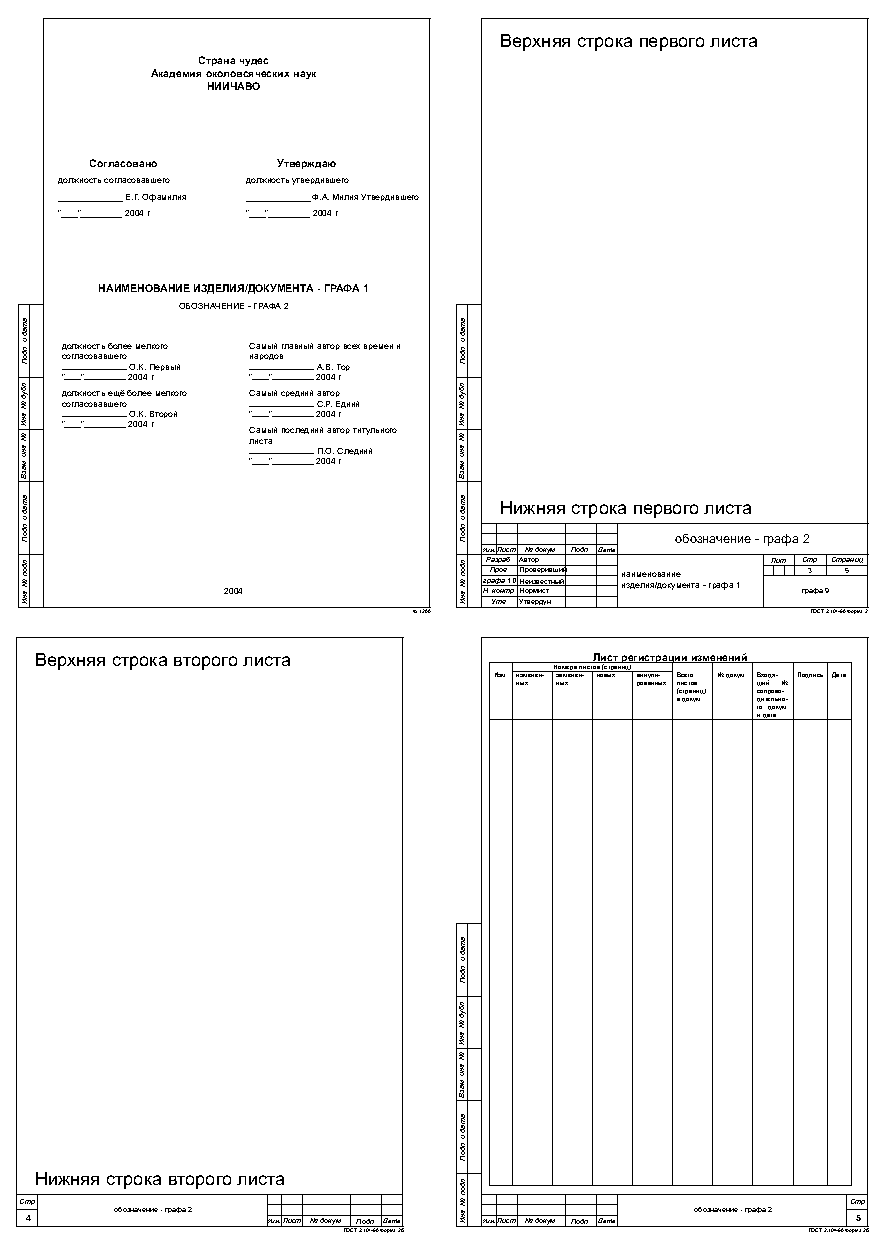
\includegraphics[width=3.5in]{example.eps}
         \end{center}
         \caption{Un esempio \textsf{psfrag}.}
    \end{figure}
\end{verbatim}
Notare l'uso di un ambiente |picture| all'interno della sostituzione
per |p1|.

\begin{figure}[tbh]
    \unitlength=1in
    \begin{center}
        \psfragscanon
        \psfrag{p1}[l]{\begin{picture}(0,0)
            \put(0.15, 0.2){\makebox(0,0)[l]{$\sin(t)$}}
            \put(0.1,0.2){\vector(-1,-2){0.1}}
            \end{picture}}
        \psfrag*{p1}[][l]{$\ast$}
        \psfrag{p2}[][l]{$\ast$}
        \psfrag{p3}{$\cos(t)$}
        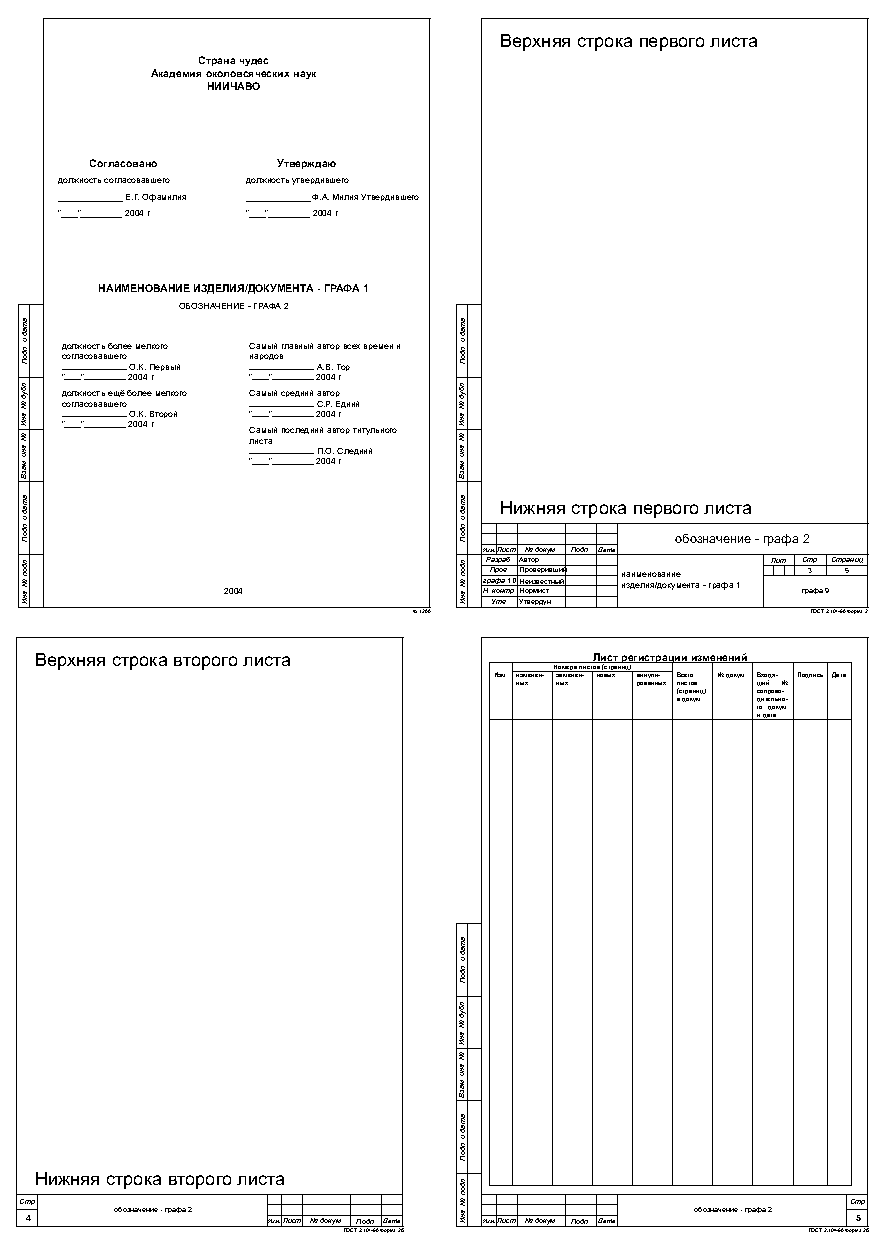
\includegraphics[width=3.5in]{example.eps}
   \end{center}
   \caption{Un esempio \pfg.}
   \label{fig:example1}
\end{figure}
Il risultato di questi due passi \`e mostrato nella figura~\ref{fig:example1}.
\subsection{Ridimensionamento della figura}
%\subsection{Figure scaling and resizing}
\label{sec:scaling}

Ci sono due modi di ridimensionare figure EPS con il pacchetto 
 \pkg{graphics}, 
e ciascuno di essi ha un effetto diverso sulle sostituzioni \pfg. 
Chi \`e solito usare lo stile \fname{epsf.sty} \`e abituato a uno solo 
di questi comportamenti.

Usando le macro \cs{scalebox} o \cs{resizebox} di \fname{graphics.sty}, 
le sostituzioni 
\pfg\  saranno ridimensionate assieme alla figura.
Questo effetto \`e illustrato nella figura~\ref{fig:example2}.
\begin{figure}[tbh]\unitlength=1in
    \begin{center}
        \psfragscanon
        \psfrag{p1}[l]{\begin{picture}(0,0)
            \put(0.15, 0.2){\makebox(0,0)[l]{$\sin(t)$}}
            \put(0.1,0.2){\vector(-1,-2){0.1}}
            \end{picture}}
        \psfrag*{p1}[][l]{$\ast$}
        \psfrag{p2}[][l]{$\ast$}
        \psfrag{p3}{$\cos(t)$}
        \resizebox{3.5in}{!}{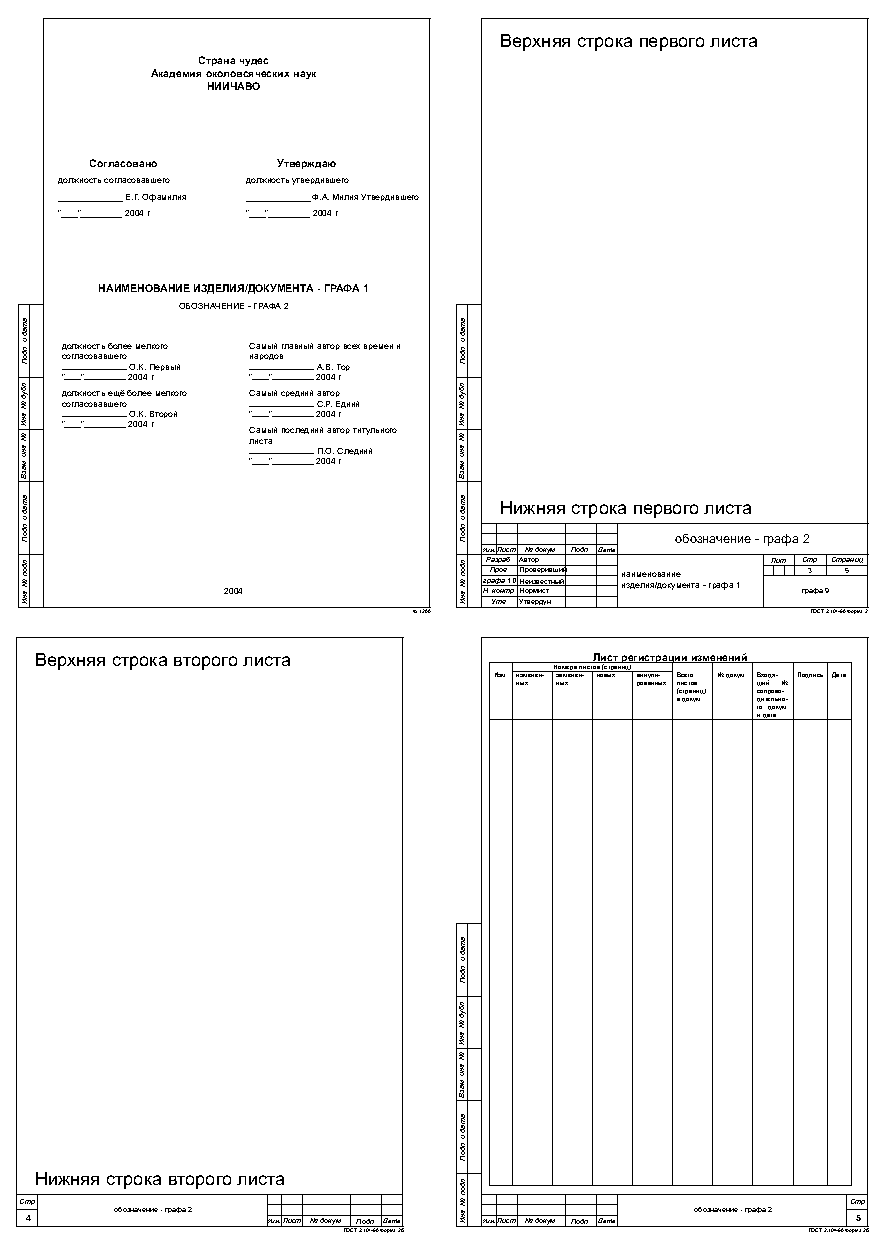
\includegraphics{example.eps}}
    \end{center}
    \caption{Lo stesso esempio \pfg\ della figura~\ref{fig:example1}, usando
             \cs{resizebox} per impostare la larghezza.}
    \label{fig:example2}
\end{figure}
L'esempio della figura~\ref{fig:example2} usa il seguente comando per portare le 
dimensioni della figura a una larghezza di 3.5 pollici:
\begin{verbatim}
\resizebox{3.5in}{!}{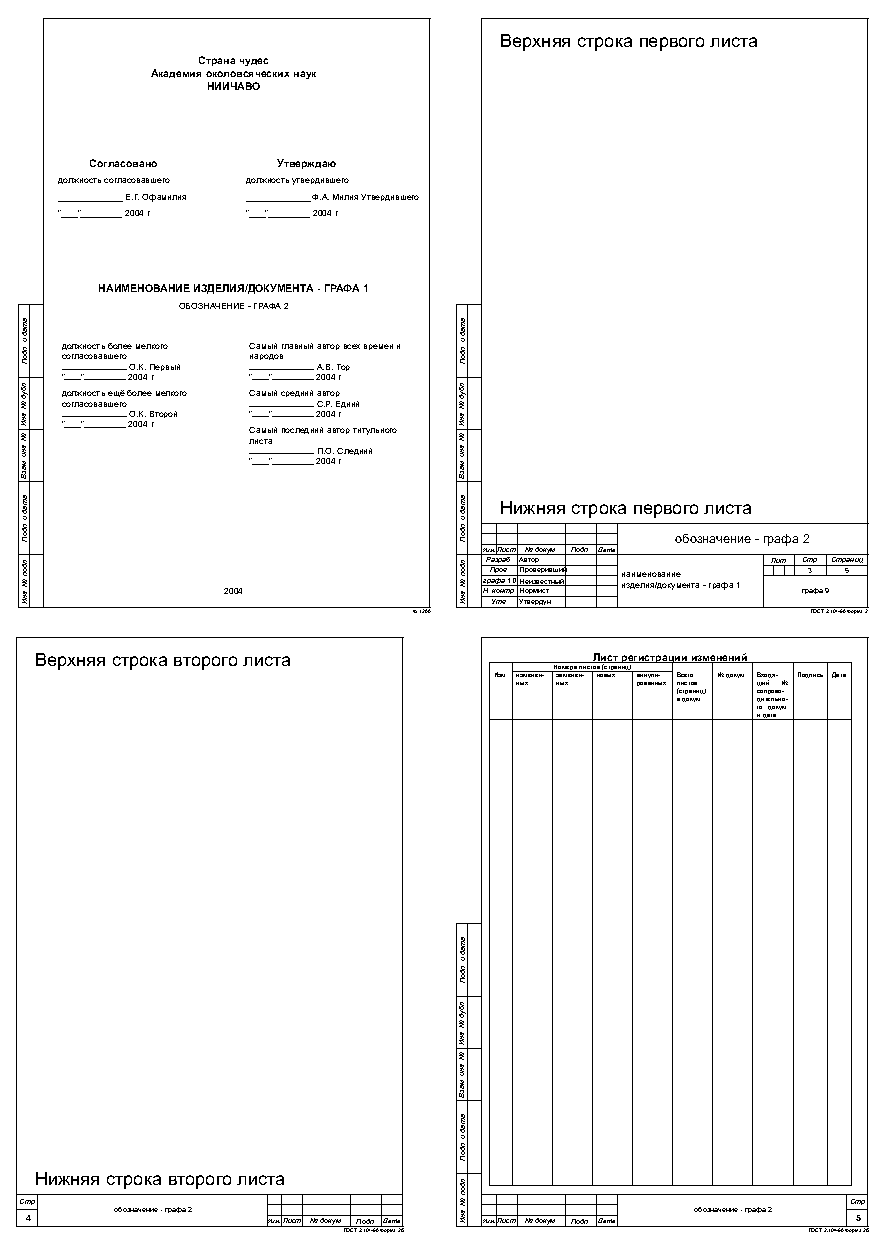
\includegraphics{example.eps}}
\end{verbatim} 
Al contrario, il codice usato per ottenere la  figura~\ref{fig:example1} usa 
la parola chiave |width=|  di \fname{graphicx.sty}:
\begin{verbatim}
\includegraphics[width=3.5in]{\includegraphics{example.eps}}
\end{verbatim}
La figura~\ref{fig:example1} illustra anche il comportamento
che si pu\`o ottenere usando le macro \fname{epsf.sty}:  \cs{epfxsize},
\cs{epsfysize}, etc. In questi casi, il testo \pfg\  non
viene ridimensionato con la figura. %to resize the figure.

Si vede chiaramente che il testo nella seconda figura \`e
pi\`u piccolo che nella prima.
Questo succede perch\'e \cs{resizebox} usa dei trucchi di PostScript per
ridimensionare tutti i contenuti del suo argomento mantenendo le proporzioni.
 Dal momento che i 
comandi \cs{psfrag} non sono realmente composti fino a quando non
si arriva all'interno del comando
\cs{includegraphics}, anch'essi vengono ridimensionati.

In \fname{graphicx.sty}, le coppie di valori chiave |width=|, |height=|,
and |scale=| ridimensionano la figura senza ridimensionare il testo che
viene sostituito, purch\'{e} siano forniti prima di un valore
per la rotazione attraverso il parametro |angle=|. Naturalmente le
macro \cs{resizebox} e \cs{scalebox}
sono ancora disponibili in \fname{graphicx.sty} quindi \`e possibile
mescolare % and match !!! 
i due comportamenti finch\'e si ottiene il risultato desiderato.
% as you see fit. !!
 
Si veda la documentazione di  \pkg{graphics} per maggiori dettagli.

Se non si \`e ancora sicuri su questa distinzione, provare entrambi i
metodi per ridimensionare le figura finch\'e non si trova una soluzione 
soddisfacente. 

\section{Errori frequenti, problemi noti, e bug}

\pfg\ \`e privo di bug.

Beh, naturalmente stiamo scherzando. \pfg\ usa alcuni trucchetti
PostScript per raggiungere i suoi obiettivi. Quindi non ci
meraviglieremmo se qualcuno dovesse trovare dei bug.  Se si riscontra
qualche problema, si controlli che non sia elencato qui sotto; se non
lo \`e, lo si segnali alla mailing list \pfg\ 
(paragrafo~\ref{sec:mail}).

\subsection{Usare correttamente i \emph{tag} di \pfg}
\label{sec:tags}

Uno dei problemi in cui gli utenti incorrono pi\`u di frequente con 
\pfg\  \`e che
alcuni \emph{tag} vengono rimpiazzati correttamente, ma non tutti. Se possibile,
quindi, bisognerebbe progettare le figure con il funzionamento di \pfg\ in mente, seguendo 
questa regola:
\begin{quote}
        Quando si aggiunge un frammento di testo (un \emph{tag}) in una figura 
        per essere sostituito da \pfg, usare una sola parola, 
        contenente solo lettere non accentate e numeri.    
\end{quote}
\pfg\  \`e stato progettato per funzionare in questo modo; 
seguire questa regola  vi d\`a la garanzia pressoch\'{e} totale 
che  \pfg\ funzioni come promesso. 
Naturalmente non \`e sempre possibile seguire questa regola, 
e un piccolo numero di pacchetti grafici d\`a costantemente dei problemi.
In tutti i casi, questi problemi possono essere risolti capendo in che modo 
 \pfg\  cerca questi \emph{tag}.

Il formato PostScript usa cinque comandi per visualizzare del testo---|show|, 
|ashow|, |kshow|, |widthshow| e |awidthshow|---anche se, in molti casi,
 un file EPS definir\`a delle abbreviazioni di questi comandi. 
\pfg, in realt\`a, intercetta questi comandi e controlla se 
contengono dei \emph{tag} da sostituire.
Quando la stringa corrisponde ad un \emph{tag} noto, 
\pfg\ si immagina dove il \emph{tag} \emph{sarebbe} stato piazzato,
e inserisce in quel punto l'opportuna sostituzione.
Se invece non trova nessuna corrispondenza, \pfg\ lascia che il comando |*show|
si comporti normalmente.

Le stringhe visualizzate dai comandi |*show| sono delimitate da parentesi, che svolgono
un ruolo simile a quello dei doppi apici nel linguaggio \fname{C}. Per esempio:
\begin{quote}
        |(Una prova.) show| ~~~~~~~~~~~~ha l'effetto di visualizzare~~~~~~~~~~~~|Una prova.|
\end{quote}
Le parentesi che non devono essere interpretate come delimitatori e 
alcuni altri caratteri speciali devono essere preceduti da un \emph{backslash} (|\|) 
in una stringa PostScript. Per esempio:
\begin{quote}
        |(x = \(0,1]) show| ~~~~~~~~~~~~visualizza~~~~~~~~~~~~|x = (0,1]|
\end{quote}

Tenendo conto di questo, ecco la regola per i \emph{tag} di \pfg:
\begin{quote}
        Il \emph{tag} passato al comando \cs{psfrag} dev'essere scritto esattamente
        come deve comparire nel comando |*show| del file EPS e senza le parentesi delimitatrici.
\end{quote}
In altre parole, \pfg\ funzioner\`a solo se la stringa nel comando \cs{psfrag} 
\`e in tutto e per tutto uguale a quanto si trova nel file EPS. Se le stringhe che si 
vogliono
sostituire contengono dei backslash, come nell'esempio di |x = \(0,1]|, allora 
si deve aggiungere un backslash anche  al comando \cs{psfrag}. \pfg, inoltre, pu\`o
sostituire solo stringhe intere, non parti di esse. Quindi se il file EPS 
contiene
\begin{quote}
        |(Voglio sostituire XXX qui) show|
\end{quote}
il comando \cs{psfrag} sbaglia se gli si passa solo |XXX|.

Volendo, si pu\`o  usare un semplice editor di testo per controllare; i file EPS, infatti, sono
(quasi sempre) solo dei semplici file ASCII.

Sfortunatamente, alcuni pacchetti grafici visualizzano il testo passando ogni carattere
singolarmente a un comando |show|. In altre parole, usando questi strumenti di disegno
per inserire la stringa ``prova'' in una figura, verr\`a prodotto un codice di questo tipo:
\begin{quote}
        |(p) show (r) show (o) show (v) show (a) show|
\end{quote}
Se lo strumento che utilizzate per produrre le figure \`e di questo tipo,
ci scusiamo; usare \pfg\ diverr\`a molto pi\`u scomodo---sar\`a
possibile usare solo \emph{tag} composti di un solo carattere. Strumenti di questo
tipo impediscono anche l'uso del comando \cs{tex}.
% seconda passata 
\subsection{Problemi nell'utilizzo di alcune figure \pkg{xfig}}

\pfg\ non funziona con le figure create con \pkg{xfig} che usano il 
 \emph{pattern fill} (``riempimento con \emph{pattern}'').
Quando si vuole colorare/riempire un poligono, \pkg{xfig} 
fornisce varie scelte possibili: 
toni di grigio, colori semplici, o alcuni riempimenti pi\`u 
complicati come ad esempio il tratteggio, \emph{checkers} (scacchiera),
etc. Purtroppo, l'uso di \emph{pattern fill} in una figura
 poi elaborata da \pfg\ 
produce dei file PostScript che non verranno stampati.

Per fortuna esistono dei metodi per aggirare questo problema:
\begin{enumerate}
        \item Non usare riempimenti a pattern nelle figure create 
        con \pkg{xfig}
        e sostituirli con colori (o con toni di grigio). 
                  Per i dettagli consultare la documentazione di \pkg{xfig}.
     
        \item Aprire il file EPS incriminato (generato da 
        \pkg{fig2dev}  o dal comando ``export'' di \pkg{xfig}) 
                con il proprio editor di testo  preferito.
                Cercare la definizione del comando \pscom{PATfill}; 
                all'interno di questa 
                subroutine, sostituire \pscom{show} com \pscom{oldshow} 
                (c'\`e una sola occorrenza).
\end{enumerate}
Un messaggio per tutti gli \emph{hacker} che modificano il codice PostScript: 
sia \pfg\ che \pkg{xfig} ridefiniscono il comando  PostScript \pscom{show}.
\pscom{oldshow} \`e il comando dove \pkg{xfig} sposta la 
``vecchia'' versione di \pscom{show}. Se riuscite a determinare
 perch\'e questo aggiustamento funziona, e convincete gli sviluppatori 
di \pkg{xfig} ad attuare questa modifica,
o se avete da suggerire un modo per correggere \pfg, per favore fatelo.

\subsection{Problemi utilizzando vecchie versioni del pacchetto \pkg{seminar}}
\label{sec:sem-bug}

Un pacchetto molto diffuso, \pkg{seminar}, \`e stato, per un certo periodo, 
incompatibile con \pfg{}
3.0. Questo \`e dovuto al fatto che \pfg{} fa affidamento su alcune 
caratteristiche della  routine di output di \LaTeXe\ , 
mentre il pacchetto \pkg{seminar} usa ancora una con molti punti in comune
con \LaTeX\ 2.09.

La migliore soluzione a questo problema \`e di assicurarsi di avere la
versione pi\`u recente del pacchetto \pkg{seminar} che si pu\`o trovare 
in ogni sito CTAN,
ad esempio nello stesso posto in cui avete trovato  \pfg. 
Una pagina web per il pacchetto \pkg{seminar}
si trova all'indirizzo \fname{http://www.tug.org/applications/Seminar/}.
La versione 13/10/1997 sembra aver corretto il problema.

Se per qualche ragione siete costretti ad usare una versione pi\`u vecchia,
esiste una soluzione temporanea, specifica per \pkg{dvips}: aggiungere il comando
|\special{header=psfrag.pro}| subito prima di |\begin{document}| nel sorgente \LaTeX.


\section{La mailing list di \pfg}
\label{sec:mail}

Esiste una mailing list Majordomo dedicata alla manutenzione di
\pfg\ndt{Attenzione, al momento della traduzione del manuale la
  mailing list di \pfg{} non \`e pi\`u attiva.}.  La mailing list
\emph{non} serve a sostituire questo manuale o a risparmiarvi una
piccola dose di congetture.  \`E invece il luogo ideale per
segnalare bug, idee per lo sviluppo, e cos\`{\i} via. Chiunque voglia
aiutare l'evoluzione di \pfg{} si pu\`o iscrivere, mandando un'email a
\begin{quote}
 \netaddress{majordomo@rascals.stanford.edu}
\end{quote}
con la riga |subscribe psfrag| nel testo dell'email.

Segnalazioni di bug, idee, etc.\ dovrebbero essere dirette a
\begin{quote}
    \netaddress{psfrag@rascals.stanford.edu}.
\end{quote}
Se trovate un bug, per favore forniteci i file
necessari (un file \LaTeX\ , le figure EPS, etc.\ in modo
che possiamo provare da soli! Provate a fornirci il p\`u piccolo
esempio indipendente che presenta il bug in questione. Se questo non \`e 
possibile, scriveteci due righe.

\end{document}




